\documentclass[11pt, oneside]{article} 
\usepackage{geometry}
\geometry{letterpaper} 
\usepackage{graphicx}
	
\usepackage{amssymb}
\usepackage{amsmath}
\usepackage{parskip}
\usepackage{color}
\usepackage{hyperref}

\graphicspath{{/Users/telliott_admin/Tex/png/}}
% \begin{center} 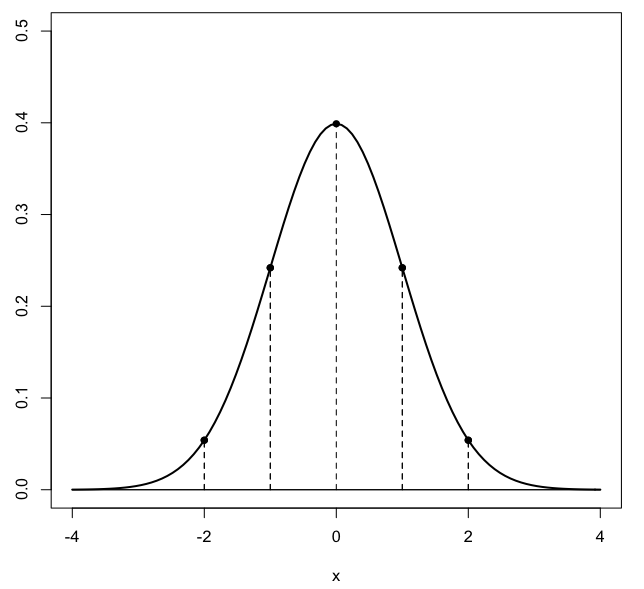
\includegraphics [scale=0.4] {gauss3.png} \end{center}

%break
\title{Cosine squared}
\date{}

\begin{document}
\maketitle
\Large

\label{sec:Cosine_squared}

This is where we solve some integrals that we put off earlier.  We already laid the groundwork by talking about trig substitutions (\hyperref[sec:Techniques_of_integration]{\textbf{here}}) and about the inverse sine function, a related topic (\hyperref[sec:Inverse_trig]{\textbf{above}}).

Let's begin with the integral of $\sqrt{1 - x^2}$.  

We saw this in the problem of the area of the circle (\hyperref[sec:Easy_pieces]{\textbf{here}}):
\[ \int \sqrt{1 - x^2} \ dx \]
We also saw it in the denominator when talking about the inverse sine
\[ \int \frac{1}{\sqrt{1 - x^2}} \ dx = \sin^{-1} x \]

To solve the first one, we use a trig substitution to give:
\[ x = \sin t \]
\[ dx = \cos t \ dt \]
\[ \sqrt{1-x^2} = \cos t \]
So
\[ \int \sqrt{1 - x^2} \ dx = \int \cos^2 t \ dt \]

We will finally solve the cosine squared in a second, but just note that the more general version of this problem has a constant, let's call it $a$:
\[ \int \sqrt{a^2 - x^2} \ dx \]
To deal with that, factor out an $a$
\[ = a \sqrt{1 - (x/a)^2} \ dx \]
Then substitute 
\[ au = x \]
 so 
 \[ a \ du = dx \]
 and we obtain
\[ = a \sqrt{1 - u^2} \ a \ du \]
\[ = a^2 \sqrt{1 - u^2}  \ du  \]

An equivalent solution is to do it during the trig substitution.

Rather than use $1$ for the hypotenuse, use the constant.  For the circle we had
\[ \int \sqrt{R^2 - x^2} \ dx \]
Let 
\[ x = R \sin t \]
\[ dx = R \cos t \ dt \]
\[ \sqrt{R^2 - x^2} = R \cos t \]
So the integral is
\[ R^2 \int \cos^2 t \ dt \]
And if you look back at that problem, I promised that we would come up with a factor of $R^2$ to make the area come out right.  Well there it is.  We still need something involving $\pi$.

It turns out the answer is 
\[ \int \cos^2 t \ dt = \frac{1}{2} \ [ \ t + \sin t \cos t \ ]  \]
We can integrate from $x = [-R,R]$.  In that case $t = [-\pi/2, \pi/2]$.  Or if we  use $0$ for the lower bound on $x$ (remembering that we'll need a factor of $2$ at the end), we will have $t = 0$ at the lower bound as well.  No matter, either way the second term with $\sin t \cos t$ will be zero.  

In the first case we'll get $\pi/2$, and in the second case we get $\pi/4$ and then multiply by $2$ to get the same thing.  Since we only did the top half of the circle we pick up another factor of $2$ for that.

\subsection*{Cosine squared}
Enough fooling around.  We want to find the integral of
\[ \int \cos^2 x \ dx \]
which as we've seen is very common in problems using trig substitution and otherwise.  The first thing to note is that 
\[ \int \sin^2 x \ dx \]
is the same problem, because
\[ \sin^2 x + \cos^2 x = 1 \]
so 
\[ \int \sin^2 x \ dx + \int \cos^2 x  \ dx = \int 1 \ dx = x \]

\subsection*{method 0}
I call this method 0 because it's not really methodical, we just guess.  If you play around differentiating products of functions (like $e^x$, $\ln x$, $\sin x$, $\cos x$ and $x$), you will soon discover that
\[ \frac{d}{dx} \ [ \ \sin x \cos x \ ] \ = \cos^2 x - \sin^2 x  \]
which can be manipulated (using $\sin^2 x + \cos^2 x = 1$) to give either
\[ \cos^2 x - \sin^2 x = 1- 2 \sin^2 x \]
or
\[ \cos^2 x - \sin^2 x = 2 \cos^2 x - 1 \]

Integrating both sides of the $\cos^2$ form we obtain
\[ \sin x \cos x = 2 \int \cos^2 x \ dx - x \]
and rearranging:
\[ \int \cos^2 x \ dx = \frac{1}{2} (x + \sin x \cos x) \]

\subsection*{method 1}
There are two other systematic approaches that can be contrasted.  The first, which is arguably the simpler one, is to remember the addition formula for cosine
\[ \cos (s+t) = \cos s \cos t - \sin s \sin t \]

As mentioned earlier, the trick I use to remember these formulas is to work out the consequences for this one:
\[ \cos (s-t) = \cos s \cos t + \sin s \sin t \]
This makes perfect sense since if $s=t$ then we get
\[ \cos 0 = \cos^2 s + \sin^2 s = 1 \]
which we know is correct.  So
\[ \cos (s+t) = \cos s \cos t - \sin s \sin t \]

If $s=t$ then (changing to $x$)
\[ \cos 2x = \cos^2 x  - \sin^2 x \]
which we saw above is equal to
\[ = 2\cos^2 x - 1 \]
The "double angle" formula is then
\[ 2 \cos^2 x = 1 + \cos 2 x \]
\[ \cos^2 x= \frac{1}{2} ( 1 + \cos 2x )  \]
Integrating
\[ \int \cos^2 x \ dx = \int \frac{1}{2} ( 1 + \cos 2x ) \ dx \]
\[ \frac{1}{2} ( x + \frac{1}{2} \sin 2x ) \]
We check by differentiating.  Leaving the factor of $1/2$ out, we obtain for $d/dx$:
\[ 1 + \cos 2x \]
which, as we saw above, is equal to $2 \cos^2 x$.  Remembering the factor of $1/2$, we obtain the expected result.

Comparing our results so far, we have obtained two different answers, namely
\[ \int \cos^2 x \ dx = \frac{1}{2} (x + \sin x \cos x) \]
\[ \int \cos^2 x \ dx = \frac{1}{2} ( x + \frac{1}{2} \sin 2x ) \]
which indicates (if there is no mistake), that
\[ \sin x \cos x = \frac{1}{2} \sin 2x  \]
to see that this is correct, recall the addition formula for sine:
\[ \sin (s+t) = \sin s \cos t + \sin t \cos s \]
then if $s=t$
\[ \sin 2s = 2 \sin s \cos s  \]

with a slight rearrangement, this is indeed what we had.

\subsection*{method 2}
In the second method, we do a substitution to take advantage of the integration by parts formula
\[ \int u \ dv = uv - \int v \ du \]
Let $u=\cos x$, so $du = -\sin x \ dx$, and let $dv = \cos x \ dx$ so $v= \sin x$, so
\[ \int \cos^2 x \ dx = \sin x \cos x + \int \sin^2 x \ dx \]

This still seems like not much progress since (as we saw) $\int \sin^2 x \ dx$ is really the same problem as $\int \cos^2 x \ dx$
\[ \int \sin^2 x \ dx = \int (1 - \cos^2 x) dx = \int dx - \int \cos^2 x dx \]

but, forging ahead, we combine the two results
\[ \int \cos^2 x \ dx = \sin x \cos x + x -  \int \cos^2 x dx \]

Rearranging:
\[ \int \cos^2 x \ dx  = \frac{1}{2} \ [ \ \sin x \cos x + x \ ] \ \]

which is what we had before.

Integration by parts where the result is a related integral can be applied to the general case of $\int \cos^n x \ dx$ with even $n$, as well as many interesting and more advanced problems.  It's worth remembering that it is in our toolbox.

\subsection*{Geometric significance}
We ran into the integral of cosine squared in looking at the area of the circle.  We'll use a unit circle to make it a bit simpler.

The integral we obtained was
\[ \int \cos^2 \theta \ d \theta = \frac{1}{2} \ [ \ \theta + \sin \theta \cos \theta \ ] \]

which can be evaluated in two ways.  We can figure out the bounds on the substituted variable $\theta$.  Since $x = \sin \theta$:
\[ x = 0 \Rightarrow \theta = 0 \]
\[ x = 1 \Rightarrow \theta = \frac{\pi}{2} \]
thus
\[ \frac{1}{2} \ [ \ \theta + \sin \theta \cos \theta \ ] \ \bigg |_0^{\pi/2} \]
and what's nice about this is the second term is zero at both the upper and lower bound, so we end up with $\pi/4$, which is correct for the quarter circle.

Or we can switch back to $x$.  We had
\[ \frac{1}{2} \ [ \ \theta + \sin \theta \cos \theta \ ] \]

Since $x = \sin \theta$, $\theta = \sin^{-1} x$ (the arc sine of $x$) so
\[ \frac{1}{2} \ [ \ \sin^{-1} x + x \sqrt{1-x^2} \ ] \]

With this approach, we can place the upper bound for this anywhere in $[0,1]$ without any trouble.

And here is where the geometry is nice.  Notice that the area under the curve can be constructed in two parts by drawing the radius to the point $(x,y)$.

\begin{center} 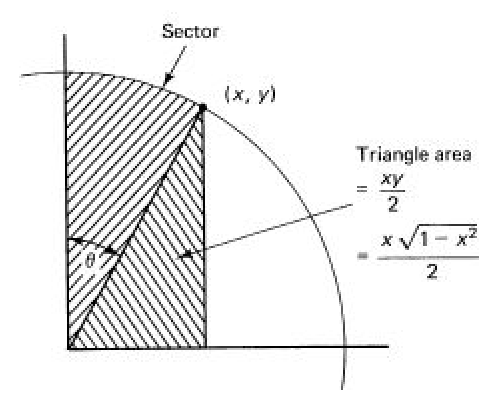
\includegraphics [scale=0.4] {circle_integral.png} \end{center}
There is a sector of the circle and a triangle.  These correspond to the two terms of
\[ \frac{1}{2} \ [ \ \sin^{-1} x + x \sqrt{1-x^2} \ ] \]
I find that very illuminating.

\subsection*{alternative parametrization}
By the way, there is another approach which gets at the close relationship between $\sin^2 \theta$ and $\cos^2 \theta$.

For a parametrized unit circle:
\[ x = \cos \theta \]
\[ dx = - \sin \theta \ d \theta \]
\[ y = \sin \theta \]
so
\[ \int y \ dx = \int -\sin^2 \theta \ d \theta \]
using the formula relating these that we had above
\[ = \int \cos^2 \theta \ d \theta - \int d \theta \]
I see this and I think, uh oh, we have an extra term here.  How will we possibly obtain the same result as before?  But it works out!

\[ = \frac{1}{2}  \ [ \ \theta + \sin \theta \cos \theta \ ] \ - \theta \]
\[ = \frac{1}{2}  \ [ \ \sin \theta \cos \theta - \theta \ ]  \]

There is another difference.  For the trig substitution we had $x = \sin \theta$, but here we have $x = \cos \theta$.  That means
\[ x = 0 \Rightarrow \theta = \frac{\pi}{2} \]
\[ x = 1 \Rightarrow \theta = 0 \]
so when we evaluate the result at these bounds we get
\[ = \frac{1}{2}  \ [ \ \sin \theta \cos \theta - \theta \ ]  \ \bigg |_{\pi/2}^0   \]
switching bounds means multiplying the expression by $-1$
\[ = \frac{1}{2}  \ [ \theta - \sin \theta \cos \theta  \ ]  \ \bigg |_0^{\pi/2}   \]

We have switched the sign on the second term ($\sin \theta \cos \theta$) --- compare with the previous answer.  But it doesn't matter because it is zero at both of the extreme bounds on the interval.  We end up with $\pi/4$, as before.

In $16.4$ Hamming turns this argument around.  He starts with the picture of the area and works backward to show that $\cos \theta$ is the derivative of $\sin \theta$ without using the limit of $\sin \theta / \theta$, which we worked out \hyperref[sec:A_famous_limit]{\textbf{here}}.


\end{document}